\section{Introdução}

\begin{frame}{Contexto}
    Analítica da Aprendizagem (Learning Analytics \textit{(LA)}): Educação, Ciência de Dados e Psicologia cognitiva.

    \begin{figure}[H]
        \centering
        \label{fig:digital_learning}
        %\caption{The data regarding the student learning process is dispersed across multiple sources} 
        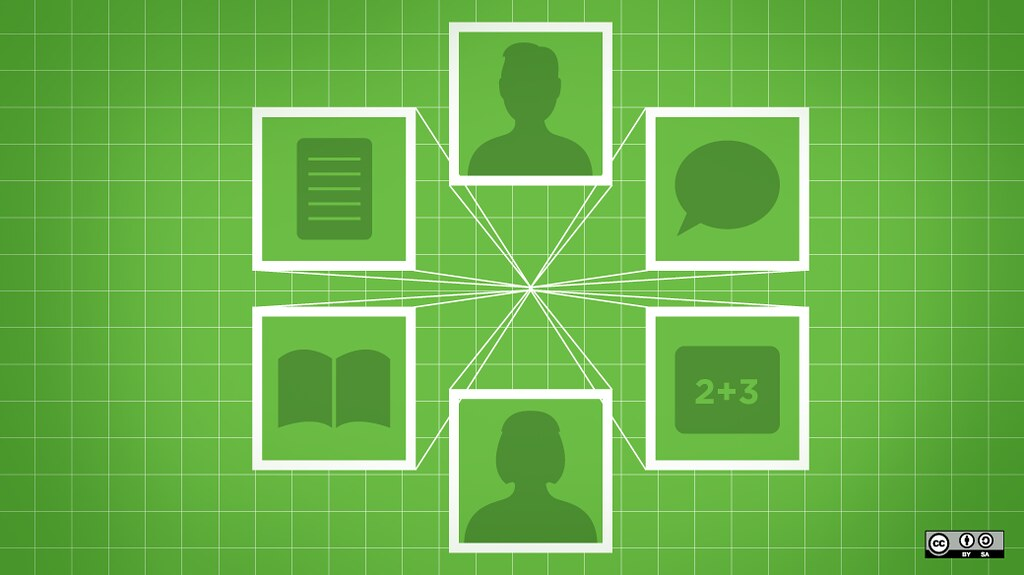
\includegraphics[width=0.5\textwidth]{../../images/digital_learning.jpg}
        \\ \small Educação: múltiplas fontes de dados
        \\ \small \url{https://www.flickr.com/photos/opensourceway/8288335386/}
    \end{figure}

    LA: Coletar, medir e interpretar dados sobre o processo de \textit{ensino e aprendizado} \cite{lang2017handbook}.
\end{frame}

\begin{frame}{Questões que cada agente educacional poderia se beneficiar com o uso de \textit{LA}}
    \begin{itemize}[<alert@+>]\color{gray}
        \item Estudantes: Querem saber seu desempenho e quais disciplinas escolher
        \item Docentes: Querem saber se sua metodologia de ensino é efetiva
        \item Técnicos: Querem saber a efetividade do suporte técnico oferecido processo de ensino e aprendizagem
        \item Gestores: Querem avaliar os cursos e desenvolver padrões de avaliação para ajudar no desenvolvimento de estratégias de mudanças
        \item Sociedade: Querem avaliar a qualidade dos profissionais que a Universidade está entregando à sociedade
    \end{itemize}
\end{frame}

\begin{frame}{Painel de Análise de Aprendizagem}
    Learning Analytics Dashboard (LAD): Informações geradas a partir de dados educacionais coletados, processados e analisados

    \begin{figure}[H]
        \centering
        \label{fig:digital_learning}
        %\caption{The data regarding the student learning process is dispersed across multiple sources} 
        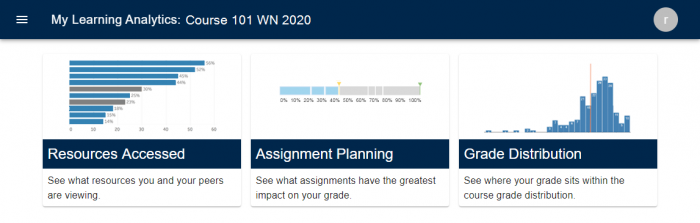
\includegraphics[width=0.8\textwidth]{../../images/myla.png}
        \\ \small My Learning Analytics - University of Michigan
        \\ \small \url{https://its.umich.edu/academics-research/teaching-learning/my-learning-analytics}
    \end{figure}
\end{frame}

\subsection{Questão de Pesquisa}
\begin{frame}{Questão de Pesquisa}
    Como a transformação do papel dos estudantes, de consumidores passivos para participantes ativos na configuração de painéis de análise de aprendizagem, aborda desafios de engenharia de software na personalização e manutenção desses painéis?
\end{frame}

